%%%%%%%%%%%%%%%%%%%%%%%%%%%%%%%%%%%%%%%%%
% Short Sectioned Assignment
% LaTeX Template
% Version 1.0 (5/5/12)
%
% This template has been downloaded from:
% http://www.LaTeXTemplates.com
%
% Original author:
% Frits Wenneker (http://www.howtotex.com)
%
% License:
% CC BY-NC-SA 3.0 (http://creativecommons.org/licenses/by-nc-sa/3.0/)
%
%%%%%%%%%%%%%%%%%%%%%%%%%%%%%%%%%%%%%%%%%

%----------------------------------------------------------------------------------------
%	PACKAGES AND OTHER DOCUMENT CONFIGURATIONS
%----------------------------------------------------------------------------------------

\documentclass[paper=a4, fontsize=11pt]{scrartcl} % A4 paper and 11pt font size

\usepackage[english]{babel}
\usepackage{graphicx}

\usepackage{color}
\definecolor{bg_text}{rgb}{0.8,0.8,0.8}
\definecolor{mygreen}{rgb}{0,0.6,0}

\usepackage{listings}
\lstset{
numbers=left,
language={},
backgroundcolor=\color{bg_text}
}


\usepackage{makeidx}
\usepackage{float}
\usepackage{color}
\usepackage[T1]{fontenc} % Use 8-bit encoding that has 256 glyphs
\usepackage{fourier} % Use the Adobe Utopia font for the document - comment this line to return to the LaTeX default
\usepackage[english]{babel} % English language/hyphenation
\usepackage{amsmath,amsfonts,amsthm} % Math packages

\usepackage{lipsum} % Used for inserting dummy 'Lorem ipsum' text into the template

\usepackage{sectsty} % Allows customizing section commands
\allsectionsfont{\centering \normalfont\scshape} % Make all sections centered, the default font and small caps

\usepackage{fancyhdr} % Custom headers and footers
\pagestyle{fancyplain} % Makes all pages in the document conform to the custom headers and footers
\fancyhead{} % No page header - if you want one, create it in the same way as the footers below
\fancyfoot[L]{} % Empty left footer
\fancyfoot[C]{} % Empty center footer
\fancyfoot[R]{\thepage} % Page numbering for right footer
\renewcommand{\headrulewidth}{0pt} % Remove header underlines
\renewcommand{\footrulewidth}{0pt} % Remove footer underlines
\setlength{\headheight}{13.6pt} % Customize the height of the header

\numberwithin{equation}{section} % Number equations within sections (i.e. 1.1, 1.2, 2.1, 2.2 instead of 1, 2, 3, 4)
\numberwithin{figure}{section} % Number figures within sections (i.e. 1.1, 1.2, 2.1, 2.2 instead of 1, 2, 3, 4)
\numberwithin{table}{section} % Number tables within sections (i.e. 1.1, 1.2, 2.1, 2.2 instead of 1, 2, 3, 4)

\setlength\parindent{0pt} % Removes all indentation from paragraphs - comment this line for an assignment with lots of text

%----------------------------------------------------------------------------------------
%	TITLE SECTION
%----------------------------------------------------------------------------------------

\newcommand{\horrule}[1]{\rule{\linewidth}{#1}} % Create horizontal rule command with 1 argument of height

\title{	
\normalfont \normalsize 
\textsc{National Institute of Technology, Goa} \\ [25pt] % Your university, school and/or department name(s)
\horrule{0.5pt} \\[0.4cm] % Thin top horizontal rule
\huge Abstractive Text Summarization \\ % The assignment title
\horrule{2pt} \\[0.5cm] % Thick bottom horizontal rule
}

\author{Dhruv Jawali, Vighnesh Birodkar \\
\\
\small{under the guidance of} \\
\\
\\
Mrs. Veena T
} % Your name

\date{\normalsize\today} % Today's date or a custom date

\begin{document}


\maketitle % Print the title
\pagebreak
\tableofcontents
\pagebreak




\section{Introduction}
\emph{Information Explosion} \cite{fshock} refers to the rapid increase in the amount of published information or data, and the effects of this abundance. The internet now consists of at least 4.3 billion web pages \cite{websize}. With each passing day, this number increases. Storing, interpreting and maintaining the ever increasing amount of information on the internet is going to be a challenge in the near future.\\
\par
Computers are ideal for storing and manipulating data, but lack the means to interpret it. Formally defining grammars for human languages is not possible, since the meanings of words are sensitive to the context. As a result, in the present scenario, the task of understanding and interpreting text data is a task primarily limitied to human subjects. Although data on the internet keeps growing exponentially, the same is neither true for the people overseeing this growth, nor for the people looking to access this information; for example, the flood of technical reviews when a new product is launched. Potential customers might have to sift through the dozens of review websites, looking for salient points in each review. It would be much easier if the information on these websites could be collected and compiled into a single, coherent document.\\
\par
Until computers are capable of interpreting human languages, humans must be kept in the loop. We need a system to limit the data the humans have to oversee, without omitting important facts. This is acheieved through \emph{Text Summarization Techniques}.\\
\par

With the current state-of-the-art in Natural Language Processing, it highly difficult, if not impossible, to design a system which derives semantic information from a text document. Hence, current text summarization techniques rely on statistical measures of importance, combined with heuristics, to assign scores to sentences within the document to create summaries. Some techniques based on forming new sentences, rather than just extracting sentences from the given set of documents, take advantage of parts-of-speech tagging, and identify semantic structure within documents. These structures, however, are limited to the type of documents being summarized, and are subject to the limitations faced by the NLP techniques used to describe them.\\
\par

An interesting way to look at the Text Summarization Problem is to pose it as a Machine Learning Problem. Using the statistical measures defined to order sentences in other extractive techniques, we model the importance of a sentence (a measure of whether it should appear in the summary or not) as a combination of these measures, and learn the weights assigned to them from human generated summaries. A regression technique is used for training, and a set of documents with summaries written by humans are used to generate scores for each sentence in the document.  In this project, we develop a novel way to generate scores for sentences in a document based on abstractive summaries written by humans, which are used to train a regression model. This model can then be used to generate extractive summaries. Evaluation of these summaries is done by generating ROUGE scores.
%TODO reference ROUGE, opinosis, radev. here
%---------------------------------------------------------------------------------------
\section{Text Summarization}
%TODO ref
Text summarization is the process of scanning a document, or a set of documents, and producing a summary which is shorter than the original document(s) which captures the important ideas expressed as much as possible. Most text summarization approaches define and try to optimize statistical criteria to select sentences from the document to be used to compose the final summary. The use of heuristics for the same is common as well.%TODO ref, read up on text summarization
Text Summarization has broadly been classified into the following two types. %TODO ref
\subsection{Extractive Text Summarization}
Given a document $D$ of $n$ sentences and a compression ratio $ 0 < r < 1 $ an \emph{Extractive Summarization Technique} selects $\lceil n \times r \rceil $  sentences which it think best represnt the document. It is called \emph{Extractive} summarization because it involves merely selecting sentences from the original document.
%TODO describe text rank and one other approach here.
\subsection{Abstractive Text Summarization}
Given a document $D$ of $n$ sentences and a compression ratio $ 0 < r < 1 $ an \emph{Abstractive Summarization Technique} produces $\lceil n \times r \rceil $  sentences which it think best represnt the document. The senteces may or may not be from the document. This approach is more likely to produce an accurate summary because it can represent facts with new and compact sentences rather than relying upon the sentences in the document. However, this requires that the summarazation technique to be grammar aware. Existing techniques implementing this approach are far from the abstractive capabilities of humans.

%TODO describe corpus and opinosis here

\section{Summarization as a Machine Learning problem}
An extractive summary can never be universal. An ideal summary can vary depending on the context and the evaluator. This is the fundamental drawback of statistical approaches. It assumes that the gist of a document can be captures by statistics alone, leaving aside the variation that comes with the reader and the context of the document.\\
\par
\emph{Machine Learning} is a technique which can take this variation into consideration. A summarizing system can be trained to optimize a different function of the document statistics depending on the context. Since purely extractive summaries are difficult to find, the system will have to be trained on abstractive summaries. Typical training data might include reviews and conclusions, papers and abstracts or movie plots and synopsis.\\
\par
Firstly we need to represent each sentence as a vector. Each component of this vector can represent a global or local feature of a sentence. The significance of a sentence in the a summary can be thought of as a function of this vector. This can be approximated by appropriate machine learning and regression techniques. \\
\par
The more complex a machine learning technique gets, the more training it requires. Purely extractive summaries are difficult to find. Heance we need a statistical measure to represent the importance of a sentence in a document given it's abstractive summary. This importance can be thought of as a function of the above mentioned vector. \\
\par
The approach can be summarized as below.\\
\\
\textbf{ Training Phase }
	\begin{itemize}
		\item Represent each sentence as a vector of features.
		\item Given a document and it's abstractive summary compute \emph{importance} of each sentence.
		\item Train a Regression Model to approximate the \emph{importance} of a sentence given it's feature vector.
	\end{itemize}

\textbf{ Prediction Phase }
	\begin{itemize}
		\item Represent each sentence as a vector of features.
		\item Used the train model to compute the \emph{importance} of a sentence.
		\item Order sentences by their \emph{importance} for the summary.
	\end{itemize}

\section{Our Approach}
\subsection{Definitions}
\textbf{\textit{Sentence}} $S$ is sequence of words $(w_1, w_2, ...... w_m )$ where $m$ is the number of words in the sentence. Length of a \textbf{\textit{Sentence}} $S$ is also abbrivated by the notation $|S|$ . For calculation purposes each word is represented by it's lowercase representation. Punctutations in sentences are not considered.\\

\textbf{\textit{Document}} $D$ is a sequence of \emph{Sentences} $(S_1, S_2, ......... S_n)$ where $n$ is the number of sentences in the document. Length of a \textbf{\textit{Document}} is also abbrivated by the notation $|D|$. \\

\textbf{\textit{Similarity}} between any two sentences $S_i$ and $S_j$ is defined as 
\begin{align}
 Similarity(S_i,S_j) =  { \cfrac{ |\{w_k | w_k \in S_i \&w_k \in S_j\}| }{log(|S_i|) + log(|S_j|)} }
\end{align}

\subsection{Importance}
To be able to train our model we need to define how important a sentence in a document is with respect to it's abstractive summary. We need a measure of how much a sentence has contributed to the summary. We do thiis by taking the maximum of similarity. We compute the similarity of a sentence in a document will all the sentences in the summary and take the maximum of all of them. So the importance of a sentence given it's summary is defined as how similar it is to the most similar sentence in the summary.\\
\par
Let $D_t$ be the Document representing the document text and $D_s$ be the document representing it's respective summary.\\

For $S_i \in D_t$ 
\begin{align}
Importance(S_i,D_s) = max(\ \{\ Similarity(S_i,S_j)\ |\ S_i \in D_s\ \}\ )  
\end{align}

An important thing to note here is that for two sentences which are mostly similar, the numberator in the expression for \emph{Similarity} increases linearly while the denominator increases logarithmically. Thus, larger sentences in the document matching larger sentences in the  summary get more significance than smaller sentences matching.\\
\par
{{\large Example}} \\
{Document Text ($D_t$)}
\begin{lstlisting}
Black Holes.
Black holes are regions from which nothing escapes.
They are formed when large stars burn out.
Black holes are incredibly dense.
Hence the escape velocity for objects is very high.
In fact, the escape velocity is faster than the speed of light.
Matter going inside a black hole is lost forever.
They can devour entire planets or stars at a time.
Black holes are found at the centre of all large galaxies.
They are difficult to observe because the do not emit light.
Black holes observed by looking at the light bent by their gravity.
\end{lstlisting}
 \vspace{1.2em}
{Summary Text ($D_s$)}
\begin{lstlisting}
Nothing can escape black holes due to the high escape velocity.
They are formed when stars die out.
They bend the light due to their graivty.
\end{lstlisting}
See Figure ~\ref{fig:importance} for a plot of importance.

\begin{figure}[h!]
  \centering
    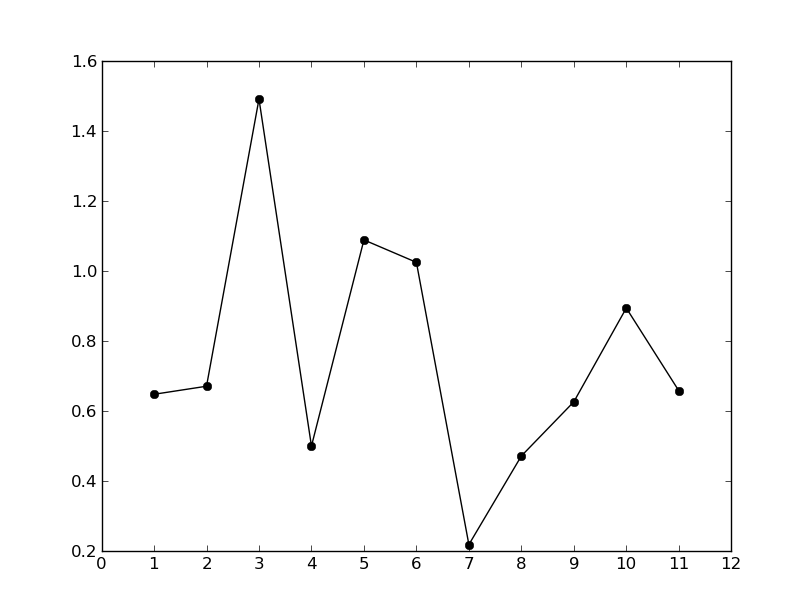
\includegraphics[width=.8\textwidth]{images/importance}
    \caption{A plot of Importance : Notice how Sentence 3 and Sentence 6 get low importance because the summary does not talk about denisty or matter being lost}
    \label{fig:importance}
\end{figure}
\pagebreak
\subsection{Sentence Features}
To be able to apply a regression technique we need to express each sentence as vector. This vector needs to capture the local as well as global significance of the sentence. For our purpose we have used the following 3 features.

\subsection{Text Rank Score}
To compute Text Rank Scores \cite{textrank} we model each sentence as a vertex in a graph. The Text Rank graph is completely connected, i.e. there is an edge connecting every two pairs of sentences. For a Document $D$, the weight between any two sentences is defined as 
\begin{align}
W( V_i,V_j) = W_{ij} = Similarity(S_i,S_j)
\end{align}

where $S_i,S_j \in D$  and $V_i,V_j$ are vertices corresponding to sentences $S_i,S_j$.\\
\\
The score for each sentence is computed as follows
\begin{align}
TR(V_i) = (1 - d)\ +\ d*\sum\limits_{V_j \in Adj(V_i)} \frac{W_{ji}}{\sum\limits_{V_k \in Adj(V_j)} W_{jk}} \times TR(V_j)
\end{align}
where $V_i$ is the vertex correcponding to Sentences $S_i$ in Document $D$, $TR(V_i)$ is the TextRank Score of $V_i$ and $Adj(V_i)$ is the set of vertices adjacent to $V_i$. $0 < d < 1$ is the damping factor and is set to $0.85$ \cite{brin}. The scores are computed repetedly till the algorithm converges. Convergence in this case is when the total update in scores over the entire graph, falls below a certain threshold. \\
\par
{\large Example}
\begin{lstlisting}
Batman - The Dark Knight.
Batman is a superhero created by DC Comics.
He strives is Gotham city to prevent crime.
Gotham city is a corrupts metropolis swarmed by criminals.
Batman in real life is Bruce Wayne.
He is a multi-millionare owner of Wayne Corp.
His gadgets and vehicles are products of Wayne Corp.
Batman has no super human capabilities.
He relies darkness and stelath for advantage.
Hence he is often called the Dark Knight.
Batman is commited ridding Gotham of crime.
\end{lstlisting}  


See Figure ~\ref{fig:tr} for a plot of Text Rank. See Figure ~\ref{fig:error} for a plot of Text Rank with iterations. 

\begin{figure}[h!]
  \centering
    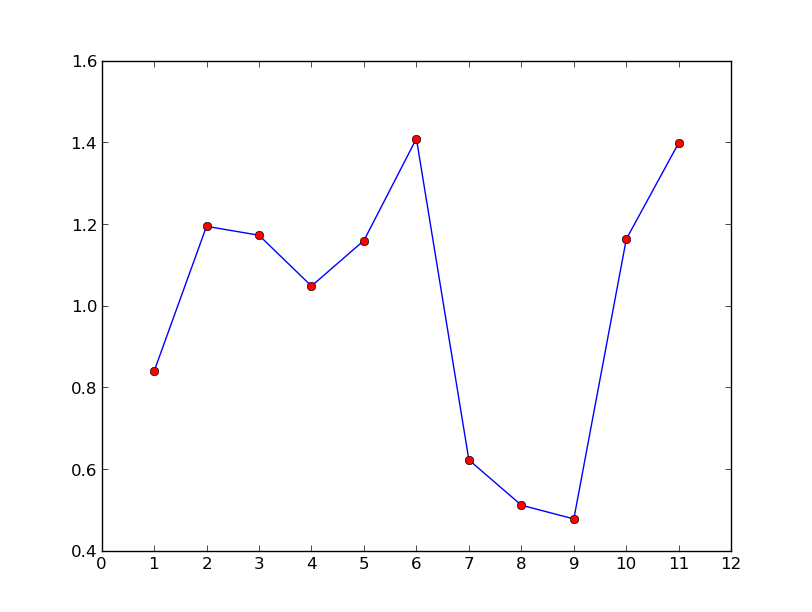
\includegraphics[width=.8\textwidth]{images/tr}
    \caption{A plot of Text Rank Scores : Notice how Sentence 6 and Sentence 11 get high Text Rank scores because they talk about Wayne Corp and Gotham, which are also talked about elsewhere}
    \label{fig:tr}
\end{figure}


\begin{figure}[h!]
  \centering
    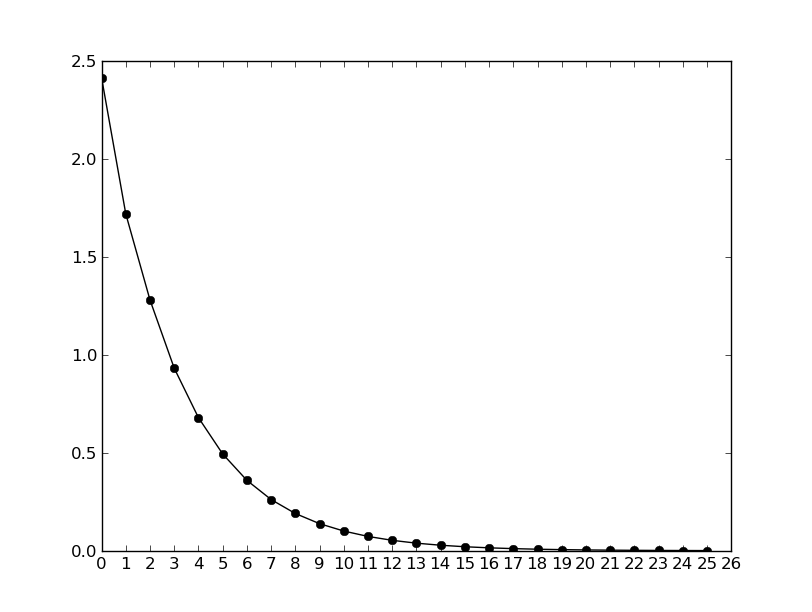
\includegraphics[width=.8\textwidth]{images/error}
    \caption{A plot of Text Rank Error : Error is the sum of magnitutdes of score updates performed}
    \label{fig:error}
\end{figure}

\pagebreak
\bibliography{report}{}
\bibliographystyle{plain}


\end{document}
